\documentclass[12pt]{article}
\usepackage{JASA_manu} %formats document like ASA wants
\usepackage{natbib} %formats citations like ASA wants
\usepackage{amssymb, amsmath, amsthm, graphics, graphicx, color, fullpage}
\usepackage{psfrag,epsf}
\usepackage{enumerate}
\usepackage{thmtools} %to format the Algorithm environment correctly
%\usepackage{hyperref}
%\hypersetup{
%  colorlinks   = true,    % Colours links instead of ugly boxes
%  urlcolor     = blue,    % Colour for external hyperlinks
%  linkcolor    = blue,    % Colour of internal links
%  citecolor    = red      % Colour of citations
%}
\usepackage{nameref, cleveref} %for named references
\usepackage[page,header]{appendix}
\usepackage{titletoc}
\usepackage{subcaption} % for subfigures

% define algorithm environment
\declaretheoremstyle[
notefont=\bfseries, notebraces={}{},
bodyfont=\normalfont\itshape,
headformat=\NAME:\NOTE
]{nopar}
\declaretheorem[style=nopar, name=Algorithm,
refname={Algorithm,Algorithms},
Refname={Algorithm,Algoritms},
numbered=no]{alg*}

\newtheorem{lem}{Lemma}

\DeclareMathOperator{\tr}{tr}
\DeclareMathOperator{\B}{B}
\DeclareMathOperator{\vech}{vech}
\DeclareMathOperator{\vect}{vec}

\graphicspath{{plots/}}

% \newcommand{\blind}{0} %uncomment for compiling separately


\begin{document}

\def\spacingset#1{\renewcommand{\baselinestretch}%
{#1}\small\normalsize} \spacingset{1}
\setlength{\tabcolsep}{2pt}

\if0\blind
{
  \title{\bf Interweaving Markov Chain Monte Carlo Strategies for Efficient
    Estimation of Dynamic Linear Models}
  \author{Matthew Simpson\\
    Departments of Statistics and Economics, Iowa State University\\~\\
    Jarad Niemi and Vivekananda Roy\\
    Department of Statistics, Iowa State University}
  \maketitle
} \fi

\if1\blind
{
  \bigskip
  \bigskip
  \bigskip
  \begin{center}
    {\LARGE\bf Interweaving Markov Chain Monte Carlo Strategies for Efficient
    Estimation of Dynamic Linear Models}
\end{center}
  \medskip
} \fi

\bigskip


\begin{abstract}
In dynamic linear models (DLMs) with unknown fixed parameters, a standard Markov chain Monte Carlo (MCMC) sampling strategy is to alternate sampling of latent states conditional on fixed parameters and sampling of fixed parameters conditional on latent states. In some regions of the parameter space, this standard data augmentation (DA) algorithm can be inefficient. To improve efficiency, we apply the interweaving strategies of \citet{yu2011center} to DLMs. For this, we introduce three novel alternative DAs for DLMs: the scaled errors, wrongly-scaled errors, and wrongly-scaled disturbances. With the latent states and the less well known scaled disturbances, this yields five unique DAs to employ in MCMC algorithms. Each DA implies a unique MCMC sampling strategy and they can be combined into interweaving and alternating strategies that improve MCMC efficiency. We assess these strategies using the local level model and demonstrate that several strategies improve efficiency relative to the standard approach and the most efficient strategy interweaves the scaled errors and scaled disturbances. Supplementary materials are available for this article online.
\end{abstract}


\noindent%
{\bf Key Words:} Ancillary augmentation; Centered parameterization; Data augmentation; Non-centered parameterization; Reparameterization; Sufficient augmentation; Time series; State-space model

\spacingset{2}

\section{Introduction}

The Data Augmentation (DA) algorithm of \citet{tanner1987calculation} and the closely related Expectation Maximization (EM) algorithm of \citet{dempster1977maximum} have become widely used strategies for computing posterior distributions and maximum likelihood estimates. While useful, DA and EM algorithms often suffer from slow convergence and a large literature has grown up around various possible improvements to both algorithms \citep{meng1997algorithm,meng1999seeking,liu1999parameter,hobert2008theoretical,yu2011center}, though much of the work on constructing improved algorithms has focused on hierarchical models \citep{gelfand1995efficient,roberts1997updating,meng1998fast,van2001art,bernardo2003non,papaspiliopoulos2007general,papaspiliopoulos2008stability}. Despite some similarities with some hierarchical models, relatively little attention has been paid to time series models, exceptions include \citet{pitt1999analytic,fruhwirth2003bayesian,fruhwirth2006auxiliary} in the DA literature and \citet{van2003one} in the EM literature. 

We seek to improve DA schemes in dynamic linear models (DLMs), i.e. linear Gaussian state-space models. The standard DA scheme uses the latent states and alternates between drawing from the full conditionals of the latent states and the model parameters \citep{fruhwirth1994data,carter1994gibbs}. The existing literature on improving DA algorithms in time series models tends to focus on non-Gaussian state-space models --- particularly the stochastic volatility model and derivative models \citep{shephard1996statistical,fruhwirth2003bayesian,roberts2004bayesian,bos2006inference,strickland2008parameterisation,fruhwirth2008heston,kastner2013ancillarity}, but a few work with the class of DLMs we consider \citep{fruhwirth2004efficient}. One recent development in the DA literature is an ``interweaving'' strategy for using two separate DAs in a single algorithm \citep{yu2011center}. This strategy draws on the strengths of both underlying DA algorithms in order to construct a Markov chain Monte Carlo (MCMC) algorithm which is at least as efficient as the worst of the two DA algorithms and, in some cases, is a dramatic improvement over the best. We implement interweaving algorithms in a general class of DLMs and, in order to do so, we introduce several new DAs for this class of models. We also show that no {\it practical} sufficient augmentation exists for the DLM, which restricts the interweaving algorithms we can construct. Using the local level model, we assess the relative performance of the various MCMC strategies.

The rest of the paper is organized as follows. In Section \ref{sec:DA}, we review the relevant DA literature and, in Section \ref{sec:DLM}, we introduce the dynamic linear model and discuss the class of DLMs we consider. In Section \ref{sec:DAs}, we introduce DAs for our class of DLMs and show that any sufficient augmentation is likely to be difficult to use. In Section \ref{sec:Algs}, we discuss the various MCMC strategies available for the DLM while Section \ref{sec:LLM} applies these algorithms to the local level model. Finally, in Section \ref{sec:Discuss}, we interpret these results and suggests directions for further research.

\section{Variations of data augmentation}\label{sec:DA}

Let $p(\phi|y)$ be a probability density, e.g. the posterior distribution of some parameter $\phi$ given data $y$. A DA adds a parameter $\theta$ with joint distribution $p(\phi,\theta|y)$ such that $\int_{\Theta}p(\phi,\theta|y)d\theta = p(\phi|y)$ and the associated DA algorithm is a Gibbs sampler for $(\phi,\theta)$. In this DA algorithm, the next draw of $\phi$ is obtained from the current draw, $k$, as follows (implicitly conditioning on $y$):
\begin{alg*}[DA]Data Augmentation\label{alg:DA}
{\small \vspace{-.5cm}
\begin{center}
  \begin{tabular}{lll}
  $[\theta|\phi^{(k)}]$ &$\to$& $[\phi^{(k+1)}|\theta]$
\end{tabular}
\end{center}
}
\end{alg*}
\noindent where $[\theta|\phi^{(k)}]$ means a draw of $\theta$ from $p(\theta|\phi^{(k)},y)$ and analogously for $[\phi^{(k+1)}|\theta]$. Though $\theta$ may be scientifically interesting, here we view its addition as a computational construct and thus focus our attention on $\phi$. 

\subsection{Alternating and Interweaving}
One well known method of improving the efficiency of MCMC samplers is judiciously choosing the DA, an example of reparameterization (see  \citet{papaspiliopoulos2007general} and references therein). Often the DA algorithms based on two separate DAs will be efficient in separate regions of the parameter space. This property suggests combining the two such DA algorithms to construct an improved sampler. One intuitive approach is to alternate between the two augmentations within a Gibbs sampler \citep{papaspiliopoulos2007general}. With two DAs $\theta$ and $\gamma$, the alternating algorithm for sampling from $p(\phi|y)$ is:
\begin{alg*}[Alt]Alternating Algorithm\label{alg:Alt}
{\small \vspace{-.5cm}
  \begin{center}
    \begin{tabular}{lllllll}
  $[\theta|\phi^{(k)}]$& $\to$& $[\phi|\theta]$& $\to$& $[\gamma|\phi]$& $\to$& $[\phi^{(k+1)}|\gamma]$.
    \end{tabular}
  \end{center}
}
\end{alg*}
\noindent One iteration of the alternating algorithm consists of an iteration of the DA algorithm based on $\theta$ followed by one iteration of the DA algorithm based on $\gamma$. 

Another option is to {\it interweave} the two DAs together \citep{yu2011center}. A global interweaving strategy (GIS) using $\theta$ and $\gamma$ as DAs is:
\begin{alg*}[GIS]Global Interweaving Strategy\label{alg:GIS}
{\small \vspace{-.5cm}
\begin{center}
\begin{tabular}{lllll}
    $[\theta|\phi^{(k)}]$ & $\to$& $[\gamma|\theta]$& $\to$& $[\phi^{(k+1)}|\gamma]$.
\end{tabular}
\end{center}
}
\end{alg*}
\noindent The GIS algorithm obtains the next iteration of the parameter $\phi$ in three steps: 1) draw $\theta$ conditional on $\phi^{(k)}$, 2) draw $\gamma$ conditional on $\theta$, and 3) draw $\phi^{(k+1)}$ conditional on $\gamma$. %This looks similar to the usual DA algorithm except a second DA is ``weaved'' in between the draw of the first DA and of the parameter. 
The second step of the GIS algorithm is often accomplished by sampling $\phi|\theta$ and then $\gamma|\theta,\phi$. This expanded GIS algorithm is:
\begin{alg*}[eGIS]Expanded GIS\label{alg:eGIS}
{\small \vspace{-.5cm}
  \begin{center}
    \begin{tabular}{lllllll}
      $[\theta|\phi^{(k)}]$& $\to$& $[\phi|\theta]$& $\to $&$[\gamma|\theta,\phi]$& $\to$& $[\phi^{(k+1)}|\gamma]$.
    \end{tabular}
  \end{center}
}
\end{alg*}
\noindent
In addition, $\gamma$ and $\theta$ are often, but not always, one-to-one transformations of each other conditional on $(\phi,y)$, i.e. $\gamma = M(\theta;\phi,y)$ where $M(.;\phi,y)$ is one-to-one, and thus $[\gamma|\theta,\phi]$ is deterministic. The key difference between the \nameref{alg:GIS} and \nameref{alg:Alt} algorithms is in step 3: instead of drawing from $p(\gamma|\phi,y)$, the GIS algorithm draws from $p(\gamma|\theta,\phi,y)$. The interweaving algorithm connects the two DAs together while the alternating algorithm keeps them separate. The weaker the dependence between the two DAs in their joint posterior, the weaker the dependence in the GIS chain and the more efficient the GIS algorithm \citep{yu2011center}. In fact with \emph{a posteriori} independent DAs, the GIS algorithm obtains iid draws from $\phi$'s posterior. Thus, we can control the dependence by choosing the two DAs carefully. 

If $\theta$ is a DA such that $p(y|\theta,\phi)=p(y|\theta)$, then $\theta$ is a {\it sufficient augmentation} (SA) for $\phi$, while if $\theta$ is a DA such that $p(\theta|\phi)=p(\theta)$, then $\theta$ is an {\it ancillary augmentation} (AA) for $\phi$ \citep{yu2011center}. In the literature, an SA is sometimes called a centered augmentation or centered parameterization while an AA is sometimes called a non-centered augmentation or non-centered parameterization. A GIS approach where one of the DAs is an SA and the other is an AA is called an ancillary sufficient interweaving strategy (ASIS). Like \citet{yu2011center} we prefer the SA and AA terminology because it suggests a connection with Basu's theorem \citep{basu1955statistics}. Under the theorem's conditions an SA and an AA are independent conditional on the model parameter, which suggests that the dependence between the two DAs will be limited in the posterior. \citet{yu2011center} show that when the group structure required to define the optimal PX-DA algorithm \citep{liu1999parameter} is present, ASIS and optimal PX-DA are equivalent.

In addition to GIS, it is possible to define a componentwise interweaving strategy (CIS) that interweaves within specific steps of a Gibbs sampler as well. A CIS algorithm for $\phi=(\phi_1, \phi_2)$ essentially employs interweaving for each block of $\phi$ separately, e.g.
\begin{alg*}[CIS]Componentwise Interweaving Strategy\label{alg:CIS}
{\small \vspace{-.5cm}
  \begin{center}
    \begin{tabular}{llllll}
      $[\theta_1|\phi_1^{(k)},\phi_2^{(k)}]$ & $\to$  & $[\gamma_1|\phi_2^{(k)},\theta_1]$ & $\to$ & $[\phi_1^{(k+1)}|\phi_2^{(k)},\gamma_1]$ &$\to$ \\
      $[\theta_2|\phi_1^{(k+1)},\phi_2^{(k)},\gamma_1]$ &$\to$ & $[\gamma_2|\phi_1^{(k+1)},\theta_2]$ & $\to$ & $[\phi_2^{(k+1)}|\phi_1^{(k+1)},\gamma_2]$ &
    \end{tabular}
  \end{center}
}
\end{alg*}\noindent
where $\theta_i$ and $\gamma_i$ are distinct data augmentations for $i=1,2$, but potentially $\gamma_1=\theta_2$  or $\gamma_2=\theta_1$. The first row draws $\phi_1$ conditional on $\phi_2$ using interweaving in a Gibbs step, while the second row does the same for $\phi_2$ conditional on $\phi_1$. The algorithm can easily be extended to additional blocks within $\phi$. CIS is attractive because it is often easier to find an AA--SA pair of DAs for $\phi_1$ conditional on $\phi_2$ and another pair for $\phi_2$ conditional on $\phi_1$ than it is to find an AA--SA pair for $\phi=(\phi_1,\phi_2)$ jointly.

\section{Dynamic linear models} \label{sec:DLM}

The general dynamic linear model is well studied \citep{harrison1999bayesian,petris2009dynamic,prado2010time} and is defined as \vspace{-.3cm}
\begin{align*}
y_t &= F_t\theta_t + v_t && v_t \stackrel{ind}{\sim} N_k(0,V_t) && (\mbox{observation equation}) \\ 
 \theta_t &= G_t\theta_{t-1} + w_t && w_t \stackrel{ind}{\sim} N_p(0,W_t) && (\mbox{system equation}) 
\end{align*}
where $N_d(\mu,\Sigma)$ is a $d$-dimensional multivariate normal distribution with mean $\mu$ and covariance $\Sigma$. The observation errors, $v_{1:T}\equiv(v_1',v_2',\dots,v_T')'$, and the system disturbances, $w_{1:T}\equiv(w_1',w_2',\dots,w_T')'$  are independent. The observed data are $y\equiv y_{1:T} \equiv (y_1',y_2',\cdots, y_T')'$ while the latent states are $\theta \equiv \theta_{0:T} \equiv (\theta_0',\theta_1',\cdots, \theta_T')'$. For each $t=1,2,\cdots,T$, $F_t$ is a $k\times p$ matrix and $G_t$ is a $p\times p$ matrix. %Let $\phi$ denote the vector of unknown parameters in the model. Then possibly $F_{t}$, $G_{t}$, $V_{t}$, and $W_{t}$ are all functions of $\phi$ for $t=1,2,\cdots,T$.

The class of DLMs we focus on sets $V_t=V$ and $W_t=W$ and treats $F_{t}$ and $G_{t}$ as known for all $t$. Our results can be extended to time varying $V_t$ or $W_t$ or to when $F_t$ or $G_t$ depend on unknown parameters, but we ignore those cases for simplicity. So $\phi=(V,W)$ is the parameter and we can write the model as \vspace{-.3cm}
\begin{align}
y_t|\theta,V,W \stackrel{ind}{\sim}  N_k(F_t\theta_t,V) \qquad \theta_t|\theta_{0:t-1},V,W  \sim  N_p(G_t\theta_{t-1},W) \label{dlmbotheqs}
\end{align}
for $t=1,2,\cdots T$. We assume the conditionally conjugate priors: $\theta_0$, $V$, and $W$ independent with $\theta_0 \sim N_p(m_0, C_0)$, $V \sim IW(\Lambda_V, \lambda_V)$ and $W \sim IW(\Lambda_W, \lambda_W)$ where $m_0$, $C_0$, $\Lambda_V$, $\lambda_V$, $\Lambda_W$, and $\lambda_W$ are known hyperparameters and $IW(\Lambda, \lambda)$ denotes the inverse Wishart distribution with degrees of freedom $\lambda$ and positive definite scale matrix $\Lambda$.

The latent states, $\theta$, can be integrated out to obtain the marginal model for the $y$: \vspace{-.3cm}
\begin{align}
  y|V,W \stackrel{ind}{\sim} N_{Tk}(D\tilde{m}, \tilde{V} + \tilde{W} + \tilde{C}). \label{margmodel}
\end{align}
where $\tilde{V}=I_T\otimes V$ where $\otimes$ is the Kronecker product, $D$ is block diagonal with elements $D_1,\ldots,D_T$, \vspace{-.2cm}
\begin{align*}
\tilde{W}_{Tk\times Tk} &= \begin{bmatrix} K_1'F_1' & K_2'F_2' & \cdots K_T'F_T' \end{bmatrix}' W \begin{bmatrix} K_1'F_1' & K_2'F_2' & \cdots K_T'F_T' \end{bmatrix}, &\\
\tilde{C}_{Tk\times Tk} &= \begin{bmatrix} H_1'F_1' & H_2'F_2' & \cdots H_T'F_T' \end{bmatrix}' C_0 \begin{bmatrix} H_1'F_1' & H_2'F_2' & \cdots H_T'F_T' \end{bmatrix},&
\end{align*}
$\tilde{m}_{Tp\times 1} = (m_0', m_0', \cdots m_0')'$. $D_t$, $K_t$, and $H_t$ are functions of the $F_t$'s and $G_t$'s and their definitions and derivations are provided in Appendix A.



\section{Augmenting the DLM}\label{sec:DAs}

In order to construct an ASIS algorithm, we need to find an SA and an AA for the DLM. \citet{papaspiliopoulos2007general} note that typically the standard DA is an SA for $\phi$ and an AA can be constructed by creating a pivotal quantity. However, the standard DA for a DLM, $\theta$, is neither an SA nor an AA. In equation \eqref{dlmbotheqs}, $V$ is in the observation equation so that $\theta$ is not an SA for $(V,W)$. Similarly $W$ is in the system equation so that $\theta$ is also not an AA for $(V,W)$. So to find an SA we need to somehow move $V$ from the observation equation to the system equation. The following lemma suggests that this will be difficult.

\begin{lem}\label{noSA}
Suppose $\eta$ is an SA for the DLM such that conditional on $\phi$, $\eta$ and $y$ are jointly normally distributed, that is
\begin{align*}
 \left. \begin{bmatrix}\eta \\ y \end{bmatrix}\right|\phi \sim N\left(\begin{bmatrix} \alpha_\eta \\ D\tilde{m} \end{bmatrix}, \begin{bmatrix}
   \Omega_\eta & \Omega_{y,\eta}' \\
   \Omega_{y,\eta} & \tilde{V} + \tilde{W} + \tilde{C} \end{bmatrix}\right).
\end{align*}
Let $A=\Omega_{y,\eta}'\Omega_{\eta}^{-1}$ and $\Sigma = \tilde{V} + \tilde{W} + \tilde{C} - A\Omega_{\eta}A'$. Then $A$, $\Sigma$, and $\alpha_{\eta}$ are constants with respect to $\phi$ and if $A'A$ is invertible, then \vspace{-.3cm}
\begin{align*}
p(\phi|\eta,y) \propto& p(y|\eta,\phi)p(\eta|\phi)p(\phi) = p(y|\eta)p(\eta|\phi)p(\phi)  \propto p(\eta|\phi)p(\phi)  \\
=& p(\phi)|(A'A)^{-1}A'(\tilde{V} + \tilde{W} + \tilde{C} - \Sigma)A(A'A)^{-1}|^{-1/2}\\
&\times \exp\left[-\frac{1}{2}(\eta - \alpha_{\eta})'[(A'A)^{-1}A'(\tilde{V} + \tilde{W} + \tilde{C} - \Sigma)A(A'A)^{-1}]^{-1}(\eta - \alpha_{\eta})\right].
\end{align*}
\end{lem}
\noindent The proof of this lemma is in Appendix B. The posterior density we wish to sample from comes from equation \eqref{margmodel} and is similar to $p(\phi|\eta,y)$ except less complicated. So what this lemma shows is that in order to use an SA in a GIS algorithm, we must sample from a density that is as hard to sample from as our target posterior. Thus if we cannot draw from the target posterior, then we cannot draw from the full conditional distribution in an SA.

While we cannot find an SA for the DLM, there are several DAs available for the construction of various MCMC algorithms. We now introduce four DAs in addition to the latent states, three of them novel.

\subsection{The scaled disturbances}\label{sec:DAs:dist}

The {\it scaled disturbances} (SDs) are constructed by creating a pivotal quantity using the system disturbances \citep{fruhwirth2004efficient}. Let $L_W$ denote the Cholesky decomposition of $W$, i.e. the lower triangular matrix $L_W$ such that $L_WL_W' =W$. Then we will define the SDs, $\gamma\equiv\gamma_{0:T}\equiv(\gamma_0',\gamma_1',\cdots,\gamma_T')'$, by $\gamma_0=\theta_0$ and $\gamma_t = L_W^{-1}(\theta_t-G_t\theta_{t-1})$ for $t=1,2,\cdots,T$. There are actually $p!$ different versions of the SDs depending on how we order the elements of $\theta_t$ but we utilize the natural ordering. 
The reverse transformation is defined recursively by $\theta_0(\gamma,L_W)=\gamma_0$ and $\theta_t(\gamma,L_W)=L_W\gamma_t + G_t\theta_{t-1}(\gamma,L_W)$ for $t=1,2,\cdots,T$. 
%The reverse transformation is defined recursively by $\theta_0=\gamma_0$ and $\theta_t=L_W\gamma_t + G_t\theta_{t-1}$ for $t=1,2,\cdots,T$. 
Using the SDs, the model is \vspace{-.3cm}
\[ y_t|\gamma,V,W  \stackrel{ind}{\sim} N_k\left(F_t\theta_t(\gamma,L_W), V\right), \qquad \gamma_t  \stackrel{iid}{\sim}N_p(0,I_p) \label{dlmdistmodel}
\]
for $t=1,2,\cdots,T$ where $I_p$ is the $p\times p$ identity matrix. Since neither $V$ nor $W$ are in the system equation, the SDs are an AA for $(V,W)$. 

\subsection{The scaled errors}\label{sec:DAs:error}
The SDs immediately suggest our first novel augmentation, called the {\it scaled errors} (SEs), i.e. $v_t=y_t - F_t\theta_t$ scaled by $V$. Let $L_V$ denote the Cholesky decomposition of $V$ so that $L_VL_V'=V$. We define the SEs as $\psi_t = L_V^{-1}(y_t - F_t\theta_t)$ for $t=1,2,\cdots,T$ and $\psi_0 = \theta_0$, although here are $k!$ versions of the SEs depending on how $y_t$ is ordered.

Assume $F_t$ is invertible for all $t$, see Appendix F of the supplementary materials and \if0\blind \citet{simpson2014app} \fi for examples of how to relax this restriction. Then $\theta_t = F_t^{-1}(y_t - L_V\psi_t)$ for $t=1,2,\cdots,T$ while $\theta_0=\psi_0$. Define $\mu_1 = L_V\psi_1 + F_1G_1\psi_0$ and $\mu_t =L_V\psi_t + F_tG_tF_{t-1}^{-1}(y_{t-1} - L_{V}\psi_{t-1})$ for $t=2,3,\cdots,T$. Then the we can write the model as \vspace{-.3cm}
\[
  y_t|V,W,\psi,y_{1:t-1} \sim N_p(\mu_t, F_tWF_t'), \qquad \psi_t  \stackrel{iid}{\sim} N_p(0,I_k)
\]
for $t=1,2,\cdots,T$ where $I_k$ is the $k\times k$ identity matrix. Since neither $V$ nor $W$ are in the system equation, the SEs are an AA for $(V,W)$. However, both $V$ and $W$ are in the observation equation so that $\psi$ is not an SA for $V|W$ nor for $W|V$.

\subsection{The ``wrongly-scaled'' DAs}
Two more novel augmentations can be obtained by scaling the SD and SE by the ``wrong'' variance so long as $F_t$ is square ($k=p$). Define $\tilde{\gamma}_t=L_V^{-1}(\theta_t - G_t\theta_{t-1})$ and $\tilde{\psi}_t=L_W^{-1}(y_t - \theta_t)$ for $t=1,2,\cdots,T$ and $\tilde{\psi}_0=\tilde{\gamma}_0=\theta_0$. We call $\tilde{\gamma}\equiv\tilde{\gamma}_{0:T}$ the {\it wrongly-scaled disturbances} (WSDs) and $\tilde{\psi}\equiv\tilde{\psi}_{0:T}$ the {\it wrongly-scaled errors} (WSEs). In terms of $\tilde{\gamma}$ the model is \vspace{-.3cm}
\[
  y_t|\tilde{\gamma},V,W \stackrel{ind}{\sim} N_p\left(F_t\theta_t(\tilde{\gamma},L_V), V\right), \qquad  
  \tilde{\gamma}_t \stackrel{ind}{\sim}N_p(0,L_V^{-1}W(L_V^{-1})')
\]
for $t=1,2,\cdots,T$ where $\theta_t(\tilde{\gamma},L_V)$ denotes the transformation from $\tilde{\gamma}$ to $\theta$ defined by the WSDs. Since $L_V$ is the Cholesky decomposition of $V$, the observation equation does not contain $W$, so $\tilde{\gamma}$ is an SA for $W|V$. Since $W$ and $L_V$ are both in the system equation, $\tilde{\gamma}$ is not an AA for $V|W$ nor for $W|V$. 

Similarly, we can write the model in terms of $\tilde{\psi}$ as \vspace{-.3cm}
\[
  y_t|V,W,\tilde{\psi},y_{1:t-1} \sim N_p(\tilde{\mu}_t, F_tWF_t'), \qquad 
  \tilde{\psi}_t  \stackrel{iid}{\sim} N_p(0,L_W^{-1}V(L_W^{-1})')
\]
for $t=1,2,\cdots,T$ where we define $\tilde{\mu}_1 = L_W\tilde{\psi}_1 - F_1G_1\tilde{\psi_0}$ and for $t=2,3,\cdots,T$ $\tilde{\mu}_t =L_W\tilde{\psi}_t - F_tG_tF_{t-1}^{-1}(y_{t-1} - L_{W}\tilde{\psi}_{t-1})$. Since $\tilde{\mu}_t$ only depends on $W$ and not on $V$, $V$ is absent from the observation equation and thus $\tilde{\psi}$ is an SA for $V|W$. Once again, since both $W$ and $V$ are in the system equation $\tilde{\psi}$ is not an AA for either $V$ or $W$.


\section{MCMC strategies for the DLM}\label{sec:Algs}

This section briefly discusses how to construct various MCMC algorithms for approximating the posterior distribution of the DLM. We focus on {\it what} to do, not {\it why}, though derivations of the relevant full conditional distributions are available in Appendix D. We occasionally come across a full conditional density that is difficult to sample from --- the details about why this happens and how to overcome it are in Appendices G and H.

\subsection{Base algorithms}\label{sec:Algs:base}
Using any of the DAs introduced in Section \ref{sec:DAs}, we can construct several DA algorithms which we call {\it base algorithms}. We will call the standard DA algorithm using $\theta$ the {\it state sampler}. In order to construct this sampler, we need to draw from two densities: $p(\theta|V,W,y)$ and $p(V,W|\theta,y)$. The latter has $V$ and $W$ independent with \vspace{-.1cm}
\[
  V|\theta,y \sim IW\left(\Lambda_V + \sum_{t=1}^Tv_tv_t',\lambda_V + T\right), \qquad
  W|\theta,y \sim IW\left(\Lambda_W + \sum_{t=1}^Tw_tw_t',\lambda_{W} + T\right), %\label{eq:VW|theta}
\]
where $v_t = y_t - F_t\theta_t$, and $w_t = \theta_t - G_t\theta_{t-1}$. 

The density $p(\theta|V,W,y)$ is multivariate normal and any algorithm to draw from it is called a simulation smoother. FFBS is the most commonly used smoother and it uses the Kalman filter \citep{fruhwirth1994data,carter1994gibbs}, but there are other options.
% \citet{koopman1993disturbance} and \citet{de1995simulation}.
We use what we are calling the mixed Cholesky factor algorithm (MCFA) to draw $\theta$ \citep{mccausland2011simulation}, also used in \citet{kastner2013ancillarity} under the name ``AWOL smoother.'' The details of this algorithm for the DLM are included in Appendix E.

Putting the pieces together, the state sampler is the following DA algorithm:
\begin{alg*}[State]State Sampler\label{alg:DLMstate}
{\small \vspace{-.5cm}
\begin{center}
\begin{tabular}{lll}
$[\theta|V^{(k)},W^{(k)}]$ & $\to$ & $[V^{(k+1)},W^{(k+1)}|\theta]$
\end{tabular}
\end{center}
}
\end{alg*}
%\begin{enumerate}
%\item Use the MCFA to sample $\theta \sim p(\theta|V,W,y)$.
%\item Sample $V \sim IW\left(\Lambda_V + \sum_{t=1}^Tv_tv_t',\lambda_V + T\right)$ and $W \sim IW\left(\Lambda_W + \sum_{t=1}^Tw_tw_t',\lambda_{W} + T\right)$ independently.
%\end{enumerate}
\noindent where the first step uses the MCFA and the second step is independent inverse Wishart draws. It is well known that this Markov chain can mix poorly in some regions of the parameter space, e.g. \citet{fruhwirth2004efficient} and Section \ref{sec:LLM}.

Next, we can use $\gamma$ in order to construct a DA algorithm called the {\it scaled disturbance sampler} or SD sampler. In the smoothing step, we need to obtain a draw from $p(\gamma|V,W,y)$. This density is also Gaussian but has a more complex precision matrix. Thus, we use the MCFA to sample $\theta \sim p(\theta|V,W,y)$ and transform from $\theta$ to $\gamma$. The density $p(V,W|\gamma,y)$ is rather complicated and does not appear easy to draw from, so we draw $V$ and $W$ in separate Gibbs steps. As a result Algorithm \nameref{alg:DLMdist} has three steps. 

\begin{alg*}[SD]Scaled Disturbance Sampler\label{alg:DLMdist}
{\small \vspace{-.5cm}
\begin{center}
\begin{tabular}{lllllll}
$[\theta|V^{(k)},W^{(k)}]$ & $\to$ & $[V^{(k+1)}|W^{(k)},\theta]$ & $\to$ & $[\gamma|V^{(k+1)},W^{(k)},\theta]$ & $\to$ & $[W^{(k+1)}|V^{(k+1)},\gamma]$
\end{tabular}
\end{center}
}
\end{alg*}
%\begin{enumerate}
%\item Use the MCFA to sample $\theta \sim p(\theta|V,W,y)$.
%\item Draw $V \sim IW\left(\Lambda_V + \sum_{t=1}^Tv_tv_t',\lambda_V + T\right)$.
%\item Transform $\theta$ to $\gamma$.
%\item Draw $W \sim p(W|V,\gamma,y)$.
%\end{enumerate}
\noindent
It is easy to show that $V|W,\gamma,y \sim IW\left(\Lambda_V + \sum_{t=1}^Tv_tv_t',\lambda_V + T\right)$ where $v_t = y_t - F_t\theta_t$ and $\theta_t$ is a function of $\gamma$ and $W$. So the first and second steps are the same draws as in Algorithm \nameref{alg:DLMstate} while the third step is a transformation from $\theta$ to $\gamma$. The last step is difficult due to the complexity of $p(W|V,\gamma,y)$, but it can be sampled from with tolerable efficiency in the local level model. In Appendix G of the supplementary materials, we have more detail as well as a rejection sampling algorithm for when $W$ is a scalar. When $W$ is a matrix it is not clear whether drawing from $p(W|V,\gamma,y)$ can be accomplished efficiently.

The DA algorithm based on the SEs is called the {\it scaled error sampler} or SE sampler (Algorithm \nameref{alg:DLMerror}) and is similar to the SD sampler with a couple of key differences. First, the simulation smoothing step in the SE sampler can be accomplished directly with the MCFA because the precision matrix of the conditional posterior of $\psi$ retains the necessary tridiagonal structure. Second, the full conditional distribution of $W$ is the familiar inverse Wishart density and the full conditional of $V$ is the complicated density. The density of $V|W,\psi,y$ is in the same class as that of $W|V,\gamma,y$. In fact there is a strong symmetry here --- the joint conditional posterior of $(V,W)$ given $\gamma$ is from the same family of densities as that of $(W,V)$ given $\psi$ so that $V$ and $W$ essentially switch places.
\begin{alg*}[SE]Scaled Error Sampler\label{alg:DLMerror}
{\small \vspace{-.5cm}
\begin{center}
\begin{tabular}{lllll}
$[\psi|V^{(k)},W^{(k)}]$ & $\to$ & $[V^{(k+1)}|W^{(k)},\psi]$ & $\to$ & $[W^{(k+1)}|V^{(k+1)},\psi]$
\end{tabular}
\end{center}
}
\end{alg*}
%\begin{enumerate}
%\item Use the MCFA to sample $\psi \sim  p(\psi|V,W,y)$
%\item Draw $V \sim p(V|W,\psi,y)$.
%\item Draw $W \sim IW\left(\Lambda_W + \sum_{t=1}^Tw_tw_t',\lambda_{W} + T\right)$.
%\end{enumerate}
\noindent The third step is the same inverse Wishart draw for $W$ as in Algorithm \nameref{alg:DLMstate}. The second step contains the difficult draw.

We can also construct DA algorithms based on the WSDs and the WSEs --- the {\it wrongly-scaled disturbance sampler} and the {\it wrongly-scaled error sampler}. In Section \ref{sec:LLM}, we show that these samplers perform poorly, so their construction is left to Appendix C. The WSDs and WSEs will ultimately be helpful in the construction of certain CIS algorithms in Section \ref{sec:Algs:CIS}.

\subsection{Alternating algorithms}\label{sec:Algs:alt}
Using the full conditionals defined in Section \ref{sec:Algs:base}, we can construct several alternating algorithms based on any two of the DAs using Algorithm \nameref{alg:Alt} on page \pageref{alg:Alt}. For example, the {\it State-SD alternating sampler} obtains the $k+1$'st iteration of $(V,W)$ from the $k$'th as follows:\vspace{-.3cm}
\begin{align*}
&[\theta|V^{(k)},W^{(k)}] \to [V^{(k+0.5)},W^{(k+0.5)}|\theta] \to\\
&[\gamma|V^{(k+0.5)},W^{(k+0.5)}] \to [V^{(k+1)}|W^{(k+0.5)},\gamma] \to [W^{(k+1)}|V^{(k+1)},\gamma].
\end{align*}
The first line is an iteration of the state sampler while the second line is an iteration of the SD sampler. No work is necessary to link up the two iterations. Each other alternating algorithm is analogous --- including algorithms using three or more DAs. %In principle, the order in which the DAs are used within an alternating algorithm could affect the convergence properties of the algorithm, but that is not investigated here. 

\subsection{GIS algorithms}\label{sec:Algs:GIS}
We can use the various DAs of Section \ref{sec:DAs} to construct GIS algorithms as well, based on Algorithm \nameref{alg:eGIS} on page \pageref{alg:eGIS}. For example, the {\it State-SD GIS sampler} is: \vspace{-.3cm}
\begin{align*}
&[\theta|V^{(k)},W^{(k)}] \to [W^{(k+0.5)},V^{(k+0.5)}|\theta] \to\\
&[\gamma|V^{(k+0.5)},W^{(k+0.5)},\theta] \to [V^{(k+1)}|W^{(k+0.5)},\gamma] \to [W^{(k+1)}|V^{(k+1)},\gamma].
\end{align*}
In the first step of the second line, we transform $\theta$ to $\gamma$ using the equations in Section \ref{sec:DAs:dist} which do not depend on V. 

There are often improvements that can be made simply by thinking clearly about what the GIS algorithm is doing. For example in the above version of the State-SD GIS sampler, the draw of $V$ in step two of line one and the draw of $V$ in step two of line two are redundant --- they come from the same distribution and only the last one is ever used in later steps. The resulting State-SD GIS sampler is as follows:
\begin{alg*}[State-SD GIS]State-Scaled Disturbance GIS Sampler
{\small \vspace{-.5cm}
\label{alg:DLMstateerror}
\begin{center}
\begin{tabular}{lllllll}
$[\theta|V^{(k)},W^{(k)}]$ & $\to$ & $[V^{(k+1)},W^{(k+0.5)}|\theta]$ & $\to$ & $[\gamma|V^{(k+1)},W^{(k+0.5)},\theta]$ & $\to$ & $[W^{(k+1)}|V^{(k+1)},\gamma]$.
\end{tabular}
\end{center}
}
\end{alg*}
%\begin{enumerate}
%\item Use the MCFA to sample $\theta \sim p(\theta|V,W,y)$.
%\item Sample $V \sim IW\left(\Lambda_V + \sum_{t=1}^Tv_tv_t',\lambda_V + T\right)$ and $W \sim IW\left(\Lambda_W + \sum_{t=1}^Tw_tw_t',\lambda_{W} + T\right)$ independently.
%\item Transform $\theta$ to $\gamma$.
%\item Sample $W \sim p(W|V,\gamma,y)$.
%\end{enumerate}
\noindent
The first two steps are both steps of Algorithm \nameref{alg:DLMstate}, the third step simply transforms from $\theta$ to $\gamma$, and the final step is the difficult draw from Algorithm \nameref{alg:DLMdist}.

Other GIS algorithms are analogous and we can construct them with three or more DAs without complication. %While the order in which we use these DAs could in principle affect mixing and convergence, like in alternating algorithms this issue is typically not important.

\subsection{CIS algorithms}\label{sec:Algs:CIS}
Next we consider CIS algorithms which have the form of Algorithm \nameref{alg:CIS} on page \pageref{alg:CIS}. The advantage of using CIS is that it is sometimes possible to find an AA-SA pair of DAs for each block of the parameter vector even when no such pair of DAs exist for the entire vector. From Section \ref{sec:DAs}, we know that the SDs and the WSDs form an AA-SA pair for $W|V$ while the SEs and the WSEs form an AA-SA pair for $V|W$.  A CIS sampler based on these AA-SA pairs obtains $(V^{(k+1)},W^{(k+1)})$ from $(V^{(k)},W^{(k)})$ as follows:
\begin{align*}
&[\psi|V^{(k)},W^{(k)}] \to [V^{(k+0.5)}|W^{(k)},\psi] \to [\tilde{\psi}|V^{(k+0.5)},W^{(k)},\psi] \to [V^{(k+1)}|W^{(k)},\tilde{\psi}]\to\\
&[\tilde{\gamma}|V^{(k+1)},W^{(k)},\tilde{\psi}] \to [W^{(k+0.5)}|V^{(k+1)},\tilde{\gamma}] \to [\gamma|V^{(k+1)},W^{(k+0.5)},\tilde{\gamma}]\to [W^{(k+1)}|V^{(k+1)},\gamma].
\end{align*}
The first line is essentially a Gibbs step for drawing $V$ that interweaves between $\psi$ and $\tilde{\psi}$ while the second line is essentially a Gibbs step for drawing $W$ that interweaves between $\gamma$ and $\tilde{\gamma}$. In the second line we use the SA before the AA in order to minimize the number of transformations we have to make in every iteration. 

Despite the fact that $\theta$, the standard augmentation, is not an SA for $V|W$, each time the WSDs or WSEs appears in the CIS sampler it would make no difference if $\theta$ was used instead because $p(V|W,\tilde{\psi},y)=p(V|W,\theta,y)$ and $p(W|V,\tilde{\gamma},y)=p(W|V,\theta,y)$. Using this we obtain a slightly different version of the CIS sampler: \vspace{-.1cm}
{\small
\begin{center}
\begin{tabular}{llllllll}
$[\psi|V^{(k)},W^{(k)}]$ & $\to$ & $[V^{(k+0.5)}|W^{(k)},\psi]$ & $\to$ & $[\psi|V^{(k+0.5)},W^{(k)},\theta]$ & $\to$ & $[V^{(k+1)}|W^{(k)},\theta]$ & $\to$ \\
$[W^{(k+0.5)}|V^{(k+1)},\theta]$ & $\to$ & $[\gamma|V^{(k+1)},W^{(k+0.5)},\theta]$ & $\to$ & $[W^{(k+1)}|V^{(k+1)},\gamma]$.&&&
\end{tabular}
\end{center}
}
\noindent We show in Appendix I that this algorithm is equivalent to SD-SE GIS in a certain sense so that we expect the mixing and convergence properties of the two algorithms to be very similar, and we confirm this in the local level model in Section \ref{sec:LLM}.

In our original definition of the CIS sampler for the DLM we used the SDs as the AA for $W$ and the SEs as the AA for $V$. We could have reversed this or used the same AA for both $V$ and $W$ since both the SEs and SDs are AAs for $(V,W)$, or we could have used $\theta$ as the AA for $V$. In each of these cases, the resulting algorithm would reduce to either the state sampler or a {\it partial CIS} algorithm \citep{yu2011center}. Appendix J discusses partial CIS algorithms in general and in the DLM. In the next section, we will characterize the efficiency of the various available samplers in the local level model (LLM).

\section{Application: The local level model}\label{sec:LLM}

The local level model is a DLM with $F_t=G_t=1$ for all $t$ while $V$ and $W$ are scalar. We can write the model as \vspace{-.3cm}
\[
  y_t |\theta,V,W \stackrel{ind}{\sim} N(\theta_t,V), \qquad
  \theta_t |\theta_{0:t-1},V,W \sim N(\theta_{t-1},W)
\]
for $t=1,2,\cdots,T$. The priors on $(\theta_0,V,W)$ from Section \ref{sec:DLM} become $\theta_0\sim N(m_0,C_0)$, $V\sim IG(\alpha_V,\beta_V)$ and $W\sim IG(\alpha_W,\beta_W)$ with $\theta_0$, $V$ and $W$ mutually independent where $IG(\alpha,\beta)$ is the inverse gamma distribution with shape parameter $\alpha$ and rate parameter $\beta$. In this model $W$ is often called the signal, $V$ the noise, and $R=W/V$ is the signal-to-noise ratio.

\subsection{DAs for the local level model}

We can define the various DAs from Section \ref{sec:DAs} in the context of the local level model. The latent states are simply $\theta$. From the states we obtain the SDs: $\gamma_0=\theta_0$ and $\gamma_t = (\theta_t - \theta_{t-1})/\sqrt{W}$ for $t=1,2,\cdots,T$. Similarly, the SEs are $\psi_0=\theta_0$ and $\psi_t = (y_t - \theta_t)/\sqrt{V}$ for $t=1,2,\cdots,T$. The WSDs are then $\tilde{\gamma}_{0}=\theta_0$ and $\tilde{\gamma}_t = (\theta_t - \theta_{t-1})/\sqrt{V}$ while the WSEs are $\tilde{\psi}_0=\theta_0$ with $\tilde{\psi}_t = (y_t - \theta_t)/\sqrt{W}$, both for $t=1,2,\cdots,T$. 

Most of the full conditional distributions required in the LLM follow straightforwardly from the general case and their derivations can be found in Appendix D. For all algorithms, we use the MCFA to draw the DA except in the case of $\gamma$, where we use MCFA to draw $\theta$ and then transform to $\gamma$. For $V$ and $W$, their draws are either an inverse gamma draw or a draw from a difficult full conditional. In Appendix D we derive the difficult density in detail and in Appendix G we show how to obtain random draws from it.

\subsection{Simulation setup}

We simulated data from the local level model using a factorial design with $V$ and $W$ each taking the values $10^{i/2}$ where $i=-4,-3,\dots,4$ and $T$ taking the values $10, 100,$ \& $1000$. For each dataset, we fit the model using a variety of the algorithms discussed above. We used the same rule for constructing priors for each model: $\theta_0\sim N(0,10^7)$, $V\sim IG(5, 4V^*)$, and $W\sim IG(5, 4W^*)$, mutually independent where $(V^*,W^*)$ are the values used to simulate the time series. The prior means are equal to $V^*$ and $W^*$ so that the prior, likelihood, and thus posterior all roughly agree about the likely values of $V$ and $W$.  This prior allows us to highlight how the behavior of each sampler depends on where the posterior is located.

For each dataset and sampler we obtained $n=10,500$ posterior draws and threw away the first $500$. The chains were started at $(V^*, W^*)$, so they can tell us about mixing but not convergence. Define the effective sample proportion for a scalar component of the chain as the effective sample size ($ESS$) \citep{gelman2013bayesian} of the component divided by the number of iterations $n$ ($ESP=ESS/n$). When $ESP=1$ the chain is behaving as if it obtains iid draws from the posterior. Occasionally $ESP>1$, if the draws are negatively correlated, but we round it down to one in our plots.

\subsection{Simulation results}

Figure \ref{fig:ESPa} contains plots of ESP for $V$ and $W$ in each chain of each base sampler for $T=100$. Let $R^*=V^*/W^*$ denote the true signal-to-noise ratio and note that the likely value of $R^*$ is highly application specific. The State sampler tends to have a low ESP for $V$ and high ESP for $W$ when $R^*>1$ with the behavior switched when $R^*<1$. The SD sampler has low ESP for both $V$ and $W$ when $R^*>1$ while the SE sampler has low ESP for both when $R^*<1$. Table \ref{tab:stnmix} summarizes the results for the base samplers on the top.

\begin{figure}[!h]
\centering
\begin{subfigure}[b]{0.59\textwidth}%
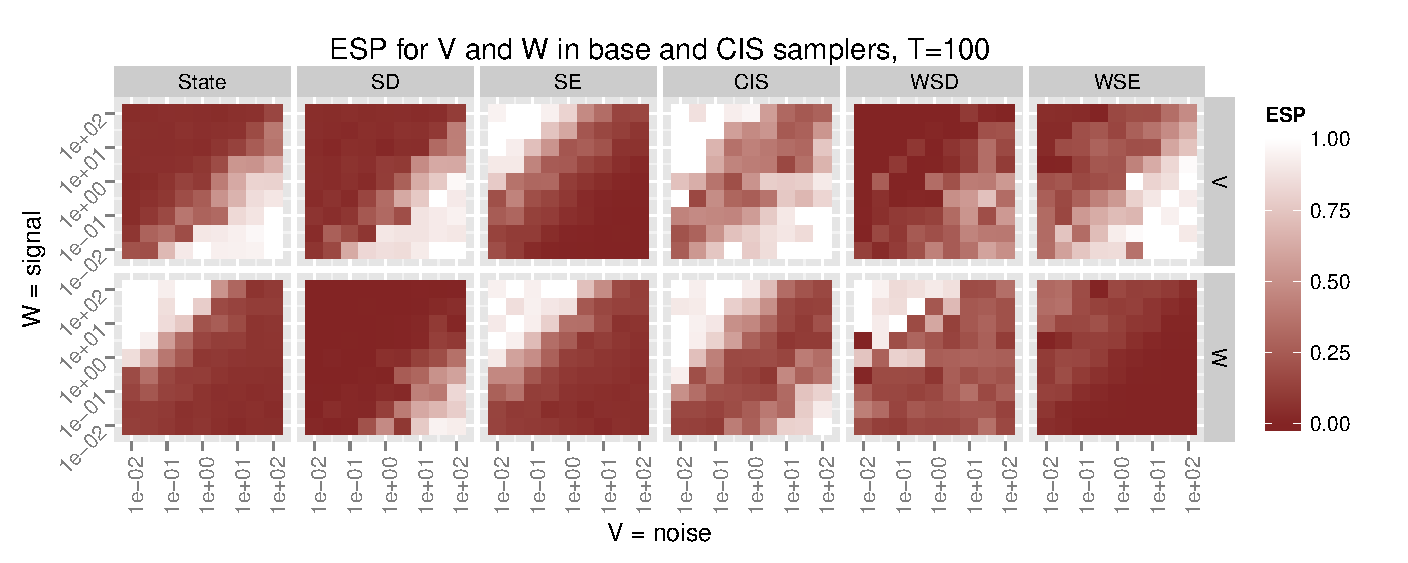
\includegraphics[width=\textwidth]{basecisESplot100}
\caption{}
\label{fig:ESPa}
\end{subfigure}
\begin{subfigure}[b]{0.53\textwidth}
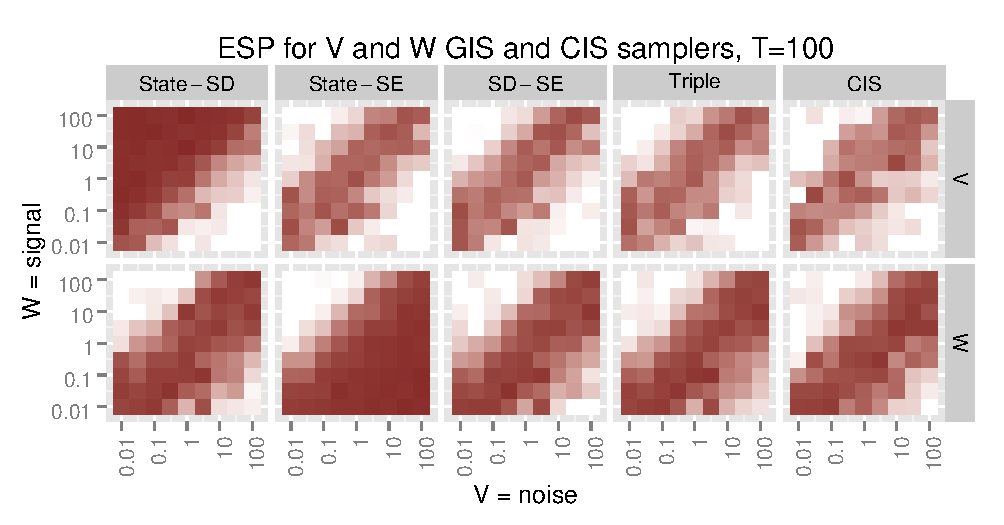
\includegraphics[width=\textwidth]{altintESplotV100}
\caption{}
\label{fig:ESPb}
\end{subfigure}
\begin{subfigure}[b]{0.45\textwidth}
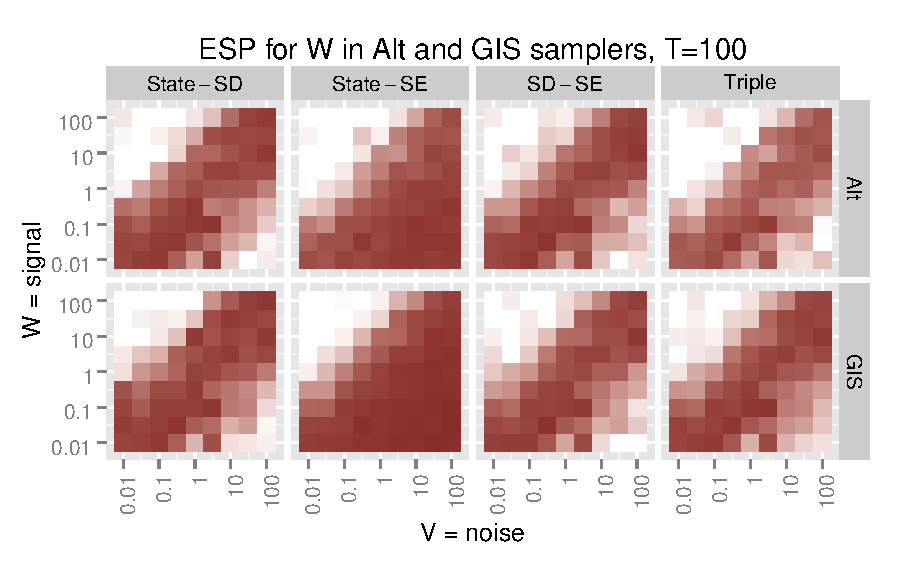
\includegraphics[width=\textwidth]{altintESplotW100}
\caption{}
\label{fig:ESPc}
\end{subfigure}
\caption{\small Effective sample proportion in the posterior sampler for a time series of length $T=100$ for $V$ and $W$ in the base sampler (a), GIS and CIS samplers (b), and Alt samplers (c). The axes indicate the true values of $V$ (horizontal) and $W$ (vertical) for the simulated data. The signal-to-noise ratio is constant moving up any diagonal. In the upper left the signal is high, in the lower right the noise is high.}
\label{ESplot}
\end{figure}

% \setlength{\tabcolsep}{6pt}
% \begin{table}
%   \centering
%   \begin{tabular}{lccccc}\hline
%      & State           & SD                 & SE                  & WSD                 & WSE \\\hline
%    V & $R^* < 1$       & $R^* < 1$           & $R^* > 1$           & $R^* < 1$           & $R^* < 1$ \\ 
%    W & $R^* > 1$       & $R^* < 1$           & $R^* > 1$           & $R^* > 1$           & $R^* > 1$ \\ \hline
%      & State-SD        & State-SE            & SD-SE              & Triple              & CIS \\\hline
%    V & $R^* < 1$       & $R^* \not\approx 1$ & $R^* \not\approx 1$ & $R^* \not\approx 1$ & $R^* \not\approx 1$ \\
%   W  &$R^* \not\approx 1$& $R^* > 1$          & $R^* \not\approx 1$ & $R^* \not\approx 1$ & $R^* \not\approx 1$\\\hline
%   \end{tabular}
%   \caption{Rule of thumb for when each sampler has a high ESP for each variable as a function of the true signal-to-noise ratio, $R^*=W^*/V^*$. The bottom panel of the table applies to both the interweaving and alternating algorithms. As the length of the time series increases, the farther away from one $R^*$ has to be for a given sampler to have a high ESP.}
%   \label{tab:stnmix}
% \end{table}


\setlength{\tabcolsep}{4pt}
\begin{table}
\small
  \centering
  \begin{tabular}{l|ccccc|ccccc}
     & State           & SD                 & SE                  & WSD                 & WSE & State-SD        & State-SE            & SD-SE              & Triple              & CIS \\\hline
   V & $R^* < 1$       & $R^* < 1$           & $R^* > 1$           & $R^* < 1$           & $R^* < 1$ & $R^* < 1$       & $R^* \not\approx 1$ & $R^* \not\approx 1$ & $R^* \not\approx 1$ & $R^* \not\approx 1$ \\ 
   W & $R^* > 1$       & $R^* < 1$           & $R^* > 1$           & $R^* > 1$           & $R^* > 1$ &$R^* \not\approx 1$& $R^* > 1$          & $R^* \not\approx 1$ & $R^* \not\approx 1$ & $R^* \not\approx 1$\\\hline
  \end{tabular}
  \caption{\small Rule of thumb for when each sampler has a high ESP for each variable as a function of the true signal-to-noise ratio, $R^*=W^*/V^*$. The right side of the table applies to both the interweaving and alternating algorithms.}
  \label{tab:stnmix}
\end{table}


We fit the model using several interweaving (GIS and CIS) samplers as well. Since the wrongly-scaled samplers behaved similarly to the state sampler and neither of the underlying DAs were an SA for $(V,W)$ jointly, we ignored them in the construction of the GIS samplers. Instead, we used the State-SD, State-SE, SD-SE, and Triple (State-SD-SE) GIS samplers, as well as the CIS sampler. Figure \ref{fig:ESPb} has plots of ESP for each of the GIS and CIS algorithms while Figure \ref{fig:ESPc} has plots of ESP for each of the Alt algorithms. Table \ref{tab:stnmix} summarizes the results on the right. 

Essentially, each GIS and Alt algorithm has high ESP when at least one of the base algorithms has high ESP. For example, the State-SD GIS and Alt algorithms have high ESP for $W$ except for a narrow band where $R^*$ is near one while ESP is high for $W$ in the state sampler when $R^*>1$ and in the SD sampler when $R^*<1$. Similarly in the State-SD GIS and Alt algorithms, mixing for $V$ is identical to the State and SD samplers since neither base sampler improves on the other in any region of the parameter space. Both the State-SD GIS and Alt algorithms take advantage of the fact that the State and SD DA algorithms make a ``beauty and the beast'' pair for $W$. However, GIS without an SA-AA pair does not appear to improve on Alt. In Section \ref{sec:Algs:CIS} we noted that the CIS and the SD-SE GIS algorithms consist of the same steps rearranged, which suggests they should perform similarly. In fact The SD-SE GIS algorithm behaves essentially identically to both the CIS and Triple GIS algorithms. 

The $T=10$ and $T=1000$ plots (Appendix M) are similar, but, as $T$ increases, the region of the parameter space with high ESP shrinks for all samplers. In Appendix K, we discuss how the pattern of correlations between various quantities in the posterior determines the pattern of ESPs in Figure \ref{ESplot}. 

In Appendix L, we also compare each algorithm based on the time required to adequately characterize the posterior, taking into account both mixing and computational time. GIS and Alt again perform essentially identical in this respect, though there is good reason to expect GIS to sometimes be more efficient. We discuss this in Appendix N and show that for very long time series, GIS does become significantly more efficient than Alt.


\section{Discussion}\label{sec:Discuss}
In order to apply the interweaving strategies of \citet{yu2011center} in DLMs we introduced five DAs, three of them novel. None of these were an SA and we argued through Lemma \ref{noSA} that it is unlikely that a {\it useful} SA exists. With available DAs, we constructed several alternating, GIS, and CIS algorithms. In a simulation study using the local level model, we tested these algorithms and found that the true signal-to-noise ratio, $R^*=V^*/W^*$, is important for determining when each algorithm performs well. In addition we found that there appears to be no difference in mixing between a GIS algorithm an its corresponding Alt algorithm for any of the DAs we used. The only caveat is that for very long time series the GIS version of an algorithm can become cheaper per iteration (Appendix N). Interweaving provides a simple framework to quickly find samplers which perform well, and for this reason we endorse the approach. As one reviewer suggested, a general strategy for constructing interweaving algorithms is as follows: implement the standard DA algorithm for each DA, find the optimal algorithm for each parameter, and combine them with the corresponding SA or AA to construct a CIS sampler. This approach yields our CIS sampler in the LLM, which along with the SD-SE GIS has the best overall performance of all the samplers we consider.

The importance of the signal-to-noise ratio to the properties of various MCMC algorithms has been anticipated in the literature. In the AR(1) plus noise model, \citet{pitt1999analytic} find that the signal-to-noise ratio with the AR(1) coefficient determine the convergence rate of a Gibbs sampler. When \citet{fruhwirth2004efficient} study the dynamic regression model with a stationary AR(1) process on the regression coefficient, they find that the relative behavior of the SD sampler and the State sampler depends on a function of the true signal-to-noise ratio that also depends on the true value of the autocorrelation parameter and the distribution of the covariate. It is likely that a version of the signal-to-noise ratio will determine how well each algorithm performs in the general DLM. This result is probably a consequence of the relevance of the Bayesian (and EM) fraction of missing information to the performance of the DA (and EM) algorithms \citep{van2001art}.

A major computational bottleneck in most of our algorithms occurs when we draw from $p(W|V,\gamma,y)$, $p(V|W,\psi,y)$, $p(V|W,\tilde{\gamma},y)$, or $p(W|V,\tilde{\psi},y)$ as discussed in Appendices G and H. The densities $p(W|V,\gamma,y)$ and $p(V|W,\psi,y)$ have the form \vspace{-0.1in}
\[ 
p(x)\propto x^{-\alpha-1}\exp\left[-ax + b\sqrt{x} - c/x\right],
\]
while the densities $p(W|V,\tilde{\psi},y)$ and $p(V|W,\tilde{\gamma},y)$ have the form \vspace{-0.1in}
\[
p(x)\propto x^{-\alpha-1}\exp\left[ -ax + b/\sqrt{x} -c/x\right]
\]
where $\alpha,a,c>0$ and $b\in\Re$. When $b=0$ we have a special case of the generalized inverse Gaussian (GIG) distribution, so perhaps the methods used to draw from a GIG can be used here. 

This difficulty could be solved by a more judicious choice of priors. We chose inverse Wishart priors for $V$ and $W$ partially because their conditional conjugacy with the states is convenient, but this breaks down when using other DAs. In addition, there are well known inferential problems with the inverse Wishart prior in the hierarchical model literature, e.g. \citet{gelman2006prior}. An alternative is the conditionally conjugate prior for $\sqrt{W}$ given the SDs. In the LLM this is a Gaussian distribution --- strictly speaking this prior is on $\pm \sqrt{W}$. If we use this prior for $\pm\sqrt{V}$ as well, the $V$ step in the SD sampler becomes a draw from the GIG distribution. This prior has been used by \citet{fruhwirth2011bayesian} and \citet{fruhwirth2008bayesian} to speed up computation while using the SDs in hierarchical models and by \citet{fruhwirth2010stochastic} for time series models with a DA similar to the SDs. We omit the results here, but using this prior on both variances does not alter our mixing results for any of the MCMC samplers.

In the general DLM this prior becomes much more complicated because $V$ and $W$ are matrices. The conditionally conjugate prior for $W$ given $\gamma$ is now a normal distribution on $L_W$, but the full conditional for the other covariance matrix becomes a matrix analogue of the GIG distribution. So no matter which conditionally conjugate prior is used, under the SEs or SDs one of $V$ or $W$'s full conditionals will be intractable. This is not a problem for the DA algorithms necessarily --- you have the freedom to use the inverse Wishart prior for $V$ and the normal prior for $L_W$ in the SD sampler, for example. But in any interweaving or alternating algorithm each covariance matrix needs to be drawn from two full conditionals, one of which will be intractable. A Metropolis step is a tolerable solution to the problem, though perhaps we can do better.

\section{Supplementary materials}\label{sec:Supp}

\begin{description}

\item[Appendices:] Provides all appendices referenced in the manuscript. (pdf file)

\item[Scripts:] Provides R scripts to run the analyses described in the manuscript, please see the \texttt{README.txt} for more details. (zip file)

\end{description}

%All supplementary materials are available in a single \verb0.zip0 file. The file \texttt{appendices.pdf} provides 8 appendices cited in the main article: A) derivation of marginal model for the DLM, B) proof of lemma 1, C) construction of the wrongly-scaled DA algorithms, D) derivations of relevant joint and full conditional distributions, E) MCFA for simulation smoothing, F) further augmentation for non-invertible $F_t$, G) efficiently drawing from $p(W|V,\gamma,y)$ and $p(V|W,\psi,y)$ in the LLM, H) efficiently drawing from $p(W|V,\tilde{\gamma},y)$ and $p(V|W,\tilde{\psi},y)$ in the LLM, I) equivalence of CIS and SD-SE GIS in the DLM, J) partial CIS Algorithms in the DLM, K) using posterior correlations to understand patterns of ESP, L) computational time for each algorithm, M) additional plots for other values of $T$, and N) comparing GIS and Alt in very long time series. The file \texttt{mcfa.R} contains R code for the MCFA smoother in the local level model. The file \texttt{dlmasisfun.R} contains R functions for obtaining simulations from a variety of MCMC algorithms in the local level model, summarizing those simulations, and for simulating data from the model. It depends on \verb0wscalerej.R0 and \verb0mcfa.R0. The file \texttt{wscalerej.R} contains several R functions for obtaining simulations from the wrongly-scaled DA algorithms in the local level model. Th e file \texttt{dlmasismixrun.R} contains R code that uses the functions in \verb0dlmasisfun.R0 and \verb0mcfa.R0 to obtain the simulations discussed in Section \ref{sec:LLM}. The file \texttt{dlmasislongrun.R} contains R code that uses the functions in \verb0dlmasisfun.R0 to obtain simulations for long time series in the local level model used in Appendix N. The file \texttt{plots.R} contains R code that uses output from \verb0dlmasismixrun.R0 to create the plots in the main document and the appendices.


\section{Acknowledgments}\label{sec:Ack}

\if0\blind{The authors thank the participants of the Economics, Finance, and Business workshop at the Bayes 250 conference and of the 2014 Bayesian Young Statisticians meeting for helpful comments, though all errors are our own. The authors would also like to thank three referees, the associated editor, and the editor for valuable comments that improved the manuscript.} \fi
\if1\blind{The authors would like to thank three anonymous reviewers and the associated editor for valuable comments that improved the manuscript.} \fi


%\clearpage
\bibliographystyle{MWS_jasa}  % proper bibliography style for ASA
\bibliography{dlmasis}
\end{document}
